\chapter{System Construction}

\section{Parallelism Analysis of Existing R\&S Procedures}

Independent is a frequently appeared modifier in literature of R\&S. Although this modifier is kept mainly for ensuring good statistical properties of sample values, it also save us much burdens redesigning simulation R\&S procedures into parallel.

However the independence is only for the simulations part. The R\&S procedure itself is completely in a serial style, namely one step is often dependent on the one prior to it. Sometimes even loops exist among steps. This serial style composes an implicit dependency chain, and becoming the potential performance bottle-neck for the whole implementation.

Now let's look into the two representative procedures we have reviewed before.

\subsection{Analysis of the Rinott's Procedure}

In the beginning part of the Rinott's procedure, things like setting up the parameters and calculating the Rinott's constant have to be done serially.

Later, sampling tasks in the initialize step, or first-stage, can be paralleled due to the independence. However, a hidden lock, or barrier lays here, since we have to wait until all the simulation experiments return its result, or sample value before we move on to the next step. Luckily to archive load balance here is quite easy.

As for the sampling tasks in the stopping step, or second-stage, it is similar to those mentioned above, only differs that the required sample numbers of different alternatives are not the same, which doesn't affect parallelism at all. Again, a implicit barrier is needed before we report the final selection.

Besides, the calculation after each barrier should be considered as the serial part of the whole program.

Anyway, Rinott's procedure is fairly easy getting paralleled and we can directly turn it into algorithm as algorithm \ref{rinott_alg}.

\begin{algorithm}
\begin{algorithmic}[1]
\Require $k, \alpha, \delta, n_0$
\State $h \gets$ the Rinott's const with arguments $k, \alpha, n_0$
\State $altIds \gets \{0, 1, 2...k - 1, 0, 1, 2...k - 1...\}$ \Comment{repeat $n_0$ cycles}
\State simulate against alternatives with id in $altIds$ \textbf{in parallel}; store result into $X_{ij}$
\State $altIds2 \gets \emptyset$
\For{$i = 0 \to k - 1$}
  \State $\bar{X_i}(n_0) = \frac{1}{n_0} \sum_{j=0}^{n_0 - 1}X_{ij}$;  $S_i^2 = \frac{1}{n_0 - 1} \sum_{j=0}^{n_0 - 1}(X_{ij} - \bar{X_i}(n_0))^2$;
  \State $N_i = \max\{n_0, \lceil \frac{h^2S_i^2}{\delta^2} \rceil\}$
  \For{$j = 0 \to (N_0 - n_0) - 1$}
    \State append $i$ into $altIds2$
  \EndFor
\EndFor
\State simulate against alternatives with id in $altIds2$ \textbf{in parallel}; store result into $X_{ij}$
\For{$i = 0 \to k - 1$}
  \State $\bar{X_i}(N_0) = \frac{1}{N_0} \sum_{j=0}^{N_0 - 1}X_{ij}$
\EndFor
\State \Return $\argmax_{i}\bar{X_i}(N_0)$
\end{algorithmic}
\caption{Rinott's Procedure}
\label{rinott_alg}
\end{algorithm}

An obvious unsatisfying issue here is the barrier laying between the two stages. Later we will modify the Rinott's procedure a little to get rid of this barrier, because essentially speaking, the existing of this barrier is due to the "sequential nature" when we describing R\&S procedures.

\subsubsection{Asynchronous Rinott's Procedure}

As can be seen easily that the calculation of each $N_i$ is independent of others. Based on this observation, we can turn the Rinott's procedure into an asynchronous style.

Generally speaking, if a program is not explicitly asynchronous, it is synchronous by default. Synchronous means when calling a function or procedure in the program, the calling statement will hang up there until the completion of the executing the called function or procedure, with return value obtained. After that, the statement right after the calling statement will start executing.

On the contrary, asynchronous means when calling a function or procedure, the calling statement will finish immediately, with input arguments passed to the called function or procedure, but with no return value obtained, and the following statement will also start its execution.

For asynchronous function call, there should be some mechanism for the caller to obtain the return value after the called function finish its execution. It could be polling, say the caller check somewhere repeatedly to see whether the result is generated, or notification, namely the called function will notify the caller when it finishes executing and the caller will take corresponding action, or precisely, execute pre-specified call-back function. Here to keep it simple we choose the polling policy, and we have another algorithm \ref{async_rinott_alg}.

\begin{algorithm}
\begin{algorithmic}[1]
\Require $k, \alpha, \delta, n_0$
\State $h \gets$ the Rinott's const with arguments $k, \alpha, n_0$
\State $altIds \gets \{0, 1, 2...k - 1, 0, 1, 2...k - 1...\}$ \Comment{repeat $n_0$ cycles}
\State simulate against alternatives with id in $altIds$ \textbf{in parallel and asynchronously}
\State $sCount \gets k \times n_0$ \Comment{sCount: sampling count}
\State initialize $count[k], sum[k], sos[k]$ \Comment{sos: sum of square}
\While {$sCount > 0$}
  \State $simOutput \gets $ take one generated simulation output; $i \gets simOutput.altId$
  \State update corresponding $count[i], sum[i], sumOfSquare[i]$; $sCount \gets sCount - 1$
  \If{$count[i] = n_0$}
	\State $mean \gets sum[i] / count[i]$; $S2 \gets (sos[i] - count[i] \times mean^2) / (count[i] - 1)$ \State $N \gets \max\{n_0, \lceil \frac{h^2S2}{\delta^2} \rceil\}$
	\If{$N > n_0$}
	  \State $altIds2 \gets \emptyset$
      \For{$j = 0 \to (N - n_0) - 1$}
        \State append $i$ into $altIds2$
      \EndFor
	  \State simulate against alternatives with id in $altIds2$ \textbf{in parallel and asynchronously}
	  \State $sCount \gets sCount + (N - n_0)$
	\EndIf
  \EndIf
\EndWhile
\State \Return $\argmax_{i} sum[i] / count[i]$
\end{algorithmic}
\caption{Asynchronous Rinott's Procedure}
\label{async_rinott_alg}
\end{algorithm}

This algorithm is identical to the previous one in mathematics, but they differ greatly in computing. In parallel computing, asynchronous execution is a common technique and we should use asynchronization where we can to reduce the serial execution in main program.

\subsection{Analysis of Fully Sequential Procedure}

Although the Rinott's procedure can get well paralleled with fairly little effort, there is still enough motivation for us to study the parallelism of fully sequential procedures, since such procedure can solve problem with potentially smaller sample size, namely total computing effort in terms of serial computing. Let's still take the one in \cite{ras-seq-jeff} as an example.

In the beginning part of this procedure, it's the same as Rinott's procedure and work here has to be done serially.

In the first-stage, it's exactly the same as Rinott's procedure, say embarrassingly parallel ends with a barrier.

However in the second-stage, things become totally different and much more interesting. Basically, the original idea is to repeat the process of taking a sample value, or running a simulation experiment, against certain alternative, then do some calculation globally to see whether some alternative can get eliminated, until there's only one alternative surviving. Let's dig out the parallelism here bit by bit.

Firstly, we don't need to run simulation experiment only one at a time, why not start as many simulation experiments as we can, as long as we do have so many task-level parallel executing units?

It looks reasonable but at least the corresponding sampling rule needs to be modified to adapt to parallel environment. Besides, even after the modification of sampling rule, another problem of the reordering of the sample obtaining sequence compared to the specified sampling sequence appears. It is due to the uncertainty of which sub-task would be finished earlier even we start these sub-tasks "at the same time" and all the executing units are "identical". The double quotes here means that it is hardly controlled by us whether these sub-tasks are started exactly at the same time and whether these executing units are exactly identical. It's not a big deal and happens in almost every parallel program, but it does become a critical issue in theoretic since it challenges the original implicit assumptions based on which the essential statistical properties are maintained.

Secondly, do we have to carry out the global calculation, or more precisely the comparison, every time after we obtain a sample value?

It should be noticed that, carrying out a global comparison will need mutual exclusive protection, otherwise the appearance of a new sample value during the comparison will make global data inconsistent for this comparative calculation. In other words, a global comparison is expensive in parallel environment.

Solutions based on decreasing comparison time sounds reasonable, but they waste elimination chances in potential. Besides, existing theory does not offer enough support.

Thirdly, can we get rid of the barrier at the end of first stage, as what we have done in the Asynchronous Rinott's procedure?

All these trouble lays on the point that the original typical fully sequential procedures are not designed specifically for parallel environment at all. It's time to revise conventional fully sequential R\&S procedure and now we will introduce two revised fully sequential procedures which are more suitable in parallel environment.

\subsubsection{Vector Filling KN Procedure}

The basic idea for vector filling KN procedure, or VFKN for short, is sticking to perform comparisons based on the originally specified sampling sequence, specified in classic KN procedure, by using an vector recording the sample values exactly in the order specified by the sampling rule. The corresponding algorithm is as algorithm \ref{vfkn_alg}.

\begin{algorithm}
\begin{algorithmic}[1]
\Require $k, \alpha, \delta, n_0$
\State $h^2 \gets (n_0 -1)[(\frac{2\alpha}{k - 1})^{-2/(n_0-1)} - 1]$
\State $altIds \gets \{0, 1, 2...k - 1, 0, 1, 2...k - 1...\}$ \Comment{repeat $n_0$ cycles}
\State simulate against alternatives with id in $altIds$ \textbf{in parallel}; store result into $X_{i\ell}$
\State $survivingCount \gets k$; $r \gets n_0$
\State comparison and elimination
\While{$survivingCount > 1$}
  \State $simOutput \gets $ take one generated simulation output into $X_{i\ell}$
  \State simulate against all surviving alternatives \textbf{in parallel and asynchronously}
  \If{$\min{len(X_i)} > r$}
    \State $r \gets r + 1$; comparison and elimination
  \EndIf
\EndWhile
\State \Return id of the surviving alternative
\end{algorithmic}
\caption{Vector Filling KN Procedure}
\label{vfkn_alg}
\end{algorithm}

The comparison and elimination here stands for a global check of inferior alternatives, namely eliminate $i$ where exist $j$ such that $\bar{X_{i\ell}}(r) - \bar{X_{j\ell}}(r) < \min\{0, -\frac{h^2S_{ij}^2}{2r\delta} + \frac{\delta}{2}\}$.

In this way, the first problem mentioned above get solved immediately with the original statistical validity staying unchanged, and the third problem is also not a big deal, since we can just consider the alternatives with sample value greater than $n_0$ when carrying out the comparison and elimination. However as for the second problem, the VFKN procedure may not use all obtained sample values at the time of each comparison, which makes it too conservative to be efficient.

And a critical implementation issue here is that essentially the VFKN procedure is to sacrifice space for statistical validity. The space here could be memory space only, with improving opportunity from self-customized memory management policy, or switching back and force from hard disks to memory if total memory space can not afford the whole vector, which will definitely slow down the computation dramatically since hard disk accessing always costs much more time than memory accessing.

\subsubsection{Asymptotic Parallel Sequential Procedure}

To over come the weaknesses in vector filling procedure, asymptotic parallel sequential procedure, or APS for short, is developed to allow unequal sample sizes for all alternatives and make elimination decisions based on all obtained sample values. In \cite{ras-seq-parallel} it has been shown that the asymptotically validity can be guaranteed as the indifference-zone parameter goes to zero. The corresponding algorithm is as algorithm \ref{aps_alg}. This time the comparison and elimination is also a global check of inferior alternatives, to eliminate $i$ where exist $j$ such that $\bar{X_{i}}(N_{ir}) - \bar{X_{j}}(N_{jr}) < \min\{0, -\frac{a}{\delta}[\frac{S_i^2(N_{ir})}{N_{ir}} + \frac{S_j^2(N_{jr})}{N_{jr}}] + \frac{\delta}{2}\}$.

\begin{algorithm}
 \begin{algorithmic}[1]
\Require $k, \alpha, \delta, n_0$
\State $a \gets - \log{[2\alpha / (k - 1)]}$
\State $altIds \gets \{0, 1, 2...k - 1, 0, 1, 2...k - 1...\}$ \Comment{repeat $n_0$ cycles}
\State simulate against alternatives with id in $altIds$ \textbf{in parallel}; store result into $X_{i\ell}$
\State $survivingCount \gets k$;
\State comparison and elimination
\State simulate against all surviving alternatives \textbf{in parallel and asynchronously}, with a phantom alternative p.
\While{$survivingCount > 1$}
  \State $simOutput \gets $ take one generated simulation output into $X_{i\ell}$
  \If{$simOutput is phantom$}
    \State simulate against all surviving alternatives \textbf{in parallel and asynchronously}, with a phantom alternative p.
    \State comparison and elimination
  \EndIf
\EndWhile
\State \Return id of the surviving alternative
 \end{algorithmic}
 \caption{Asymptotic Parallel Sequential Procedure}
 \label{aps_alg}
\end{algorithm}

Since APS procedure can almost fully utilize all the obtained sample values, it is definitely more efficient in eliminating inferior alternatives than VF. Besides, APS procedure doesn't require recording all the sample values obtained. It only needs some summarizing information of obtained sample values like summation, summation of square and so on, which can be updated as new sample value obtained. This feature lowers the storage space demand and in this way the whole data of APS procedure can be easily fit into main memory, which guarantees the order of computing speed.

\section{System Design}

With the revision of existing simulation R\&S procedures, now it is possible to implement serial ranking and selection within an architecture for parallel execution. We will adopt the master-slave pattern as the higher lever architecture for its flexibility to support features aside of embarrassingly parallel part in simulation R\&S procedures and scalability to deal with the large-scale size in selecting the best problem. Besides, it is also fairly easy from a implementation viewpoint.

\subsection{Overview}

In parallel computing, the master-slave pattern means that there is a single master execution unit dealing with the serial part while several identical slave execution units sharing the workload which can be carried out in parallel. For simulation R\&S procedures, the serial R\&S procedure should be implemented within the master, while the independent simulation experiments should be spread out among all the slaves, with explicit or implicit scheduling from the master.

\begin{figure}[ht]
\centering
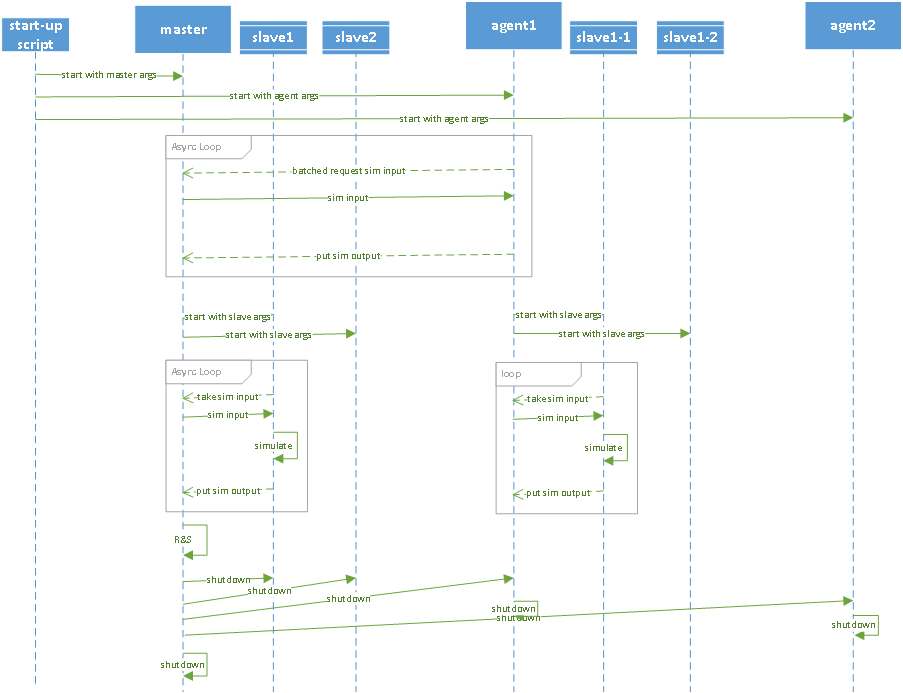
\includegraphics[width=120mm]{overview_seq.png}
\caption{Overview Sequence Diagram}
\end{figure}

The above figure is an overview sequence diagram. As it illustrates, the start-up script will firstly start the master, then the agents. The master, including all the agents, will start its local slaves. The agent here may be regarded as a secondary master, because the whole system is deployed on a cluster and some slaves have to run on different machines rather than the same machine as master, which involves network communication from some slaves to the master via their own agent.

After start-up and many trivial tasks like arguments parsing, the R\&S procedure will be running inside the master, say specifying the sampling rule, collecting the sample values and eliminating inferior alternatives based on them, until the best alternative is selected. During that time, all the slaves are doing simulation experiments again and again, against different alternatives and with different random number generation seeds.

After the whole process, extensive logs are generated and will be used in further analysis. For verification purpose, the process may be carried out more than one time.

Now, we will introduce these modules one by one.

\subsection{Slave}

Slave is the simplest module within the system and it has many different instances. A slave instance is a dedicated thread. These threads are identical in code while different in the data it is processing and the status it is in.

Briefly speaking, there are three steps inside a working cycle of slave thread, they're simulation arguments or input fetching, simulation experiment executing and simulation result or output submitting. The slave threads will follow this working cycle one round after another until explicitly stopped.

Both argument fetching step and result submitting step involve communicating with the master, or more precisely, the R\&S procedure. If the slave is not running on the same machine as the master, network communication is also involved, which is considered as extra cost introduced by adopting parallel computing. We have used two FIFO queues to buffer the input and output of simulation to reduce such communication cost. We will leave the illustration of detailed buffering policy in later part, since it's not the duty of slave.

As for the simulation step, it is done simply by calling the abstract programming interface of simulation task, thus supporting self-customized simulation experiments. To make this clear, readers should first noticed that our system can be divided into two major parts. One part includes the core components, the other consists of implementations of different R\&S procedures and different simulation experiments. Every time user of our system should choose one specific implementation of R\&S procedure and one specific implementation of simulation experiments, and start this R\&S program together with all the core components.

In other words, the core components are programmed with only dependent on the abstract function signatures of both R\&S procedures and simulation. This follows an important design rule, say, depend on abstract rather than implementation. In this way, the core component part can stay unchanged against the change of R\&S and simulation.

Since there has already been so many different combinations of R\&S procedures and simulation experiments to solve selecting the best problem, it is necessary to extract the common components and define reasonable extension points for different components, which follows an import design principle saying that "don't repeat your self". And it will also help a lot when facing a new selecting the best problem since researchers can focus on the part that the new problem differs from others, as long as the specific solution for the different part is developed strictly against the specifications of extension points stated in the rest of this section.

Now we will look detail into the abstract programming interface of simulation task.

\subsubsection{Integrating Simulation Experiment}

Here is the specification of this programming interface:

\begin{lstlisting}[language=Java]
public double[] sim(double[] alt, double[] args, long[] seed);
\end{lstlisting}

The first function parameter $alt$ is an array containing all the data needed to identify and fully describe the alternative, against which to run the simulation.

The second function parameter $args$ is an array containing the common arguments for all the simulation.

The third function parameter seed is an array of integers needed in generating uniformly distributed random numbers with the $MRG32k3a$ algorithm. The main idea here is to make each simulation against the same alternative independent from each other in the viewpoint of statistic by attaching each simulation a different set of seeds, which is generated in master as part of the simulation input. What's more, we also need a set of seeds to generate many sets of seeds used by simulation experiments, and the "master seeds" could be specified by user.

The return value is design as an array to support multiple simulation output.

Throughout the design of these extension points, we will try our best not to involve programming language dependent grammar or feature in the hope of reducing user's learning effort, just like the arrays here is plain array of double which is similar to most C-style languages, rather than advanced data structure like $ArrayList$ provided by Java standard library.

In a word, integrating customized simulation experiment into slave is quite easy. The only issue that needs attention here is to remember using the seeds provided from master reasonably during simulation.

\subsubsection{Dealing with Thread-unsafe Library}

However, the real world is not that perfect as expected. The SSJ, a famous Java library for discrete-event simulation proposed in \cite{ssj}, is not thread-safe, which means it can not guarantee correct execution within multiple threads. The reason is that it place some thread-private data into static fields of Java class, which can be accessed by all threads. To overcome this, we designed our own Java class loading policy, to reload such thread-unsafe classes inside each slave thread, such that related static fields of Java class have its own place inside each slave thread. In this way we work around temporarily, and we will leave redesigning a thread-safe library as future work.

\subsection{Master}

Master has only one instance, which is also a dedicated thread, but not exactly the main thread for the whole process, since there's more "duty" work left to do in main thread like parsing parameters of R\&S procedure, inputting the data of every alternative and other program level configurations like number of slave threads or directory for log files.

After that, some data structures are initialized, where the most important ones are two FIFO queues buffering the input and output of simulation experiments.

\subsubsection{Communication with FIFO Queues}

Direct communication among the master and slaves are quite expensive, in the sense that slaves have to take turns when communicating with master and the master itself needs to guarantee mutual exclusion, which put more burden on the single threaded master. In order to overcome this shortage, we have used FIFO queues, or $BlockingQueue$ in Java.

The FIFO queue is is a abstract data structure that all the elements are keep in order and theoretically only two operations are supported. One is enqueue, which appends one element to the end of queue, the other is dequeue, which extract one element at the beginning of the queue. Both of them have $O(1)$ complexity. In parallel environment, the enqueue operation will stuck there if the queue is full, and it's the same for dequeue operation if the queue is empty.

With FIFO queues, the master could just send out simulation parameters to a queue and obtain simulation results from another, thus won't get stuck in most cases. On the hand, slaves can receive simulation parameters from the first queue and put simulation results to the second one. Just like the figure below:

\begin{figure}[ht]
\centering
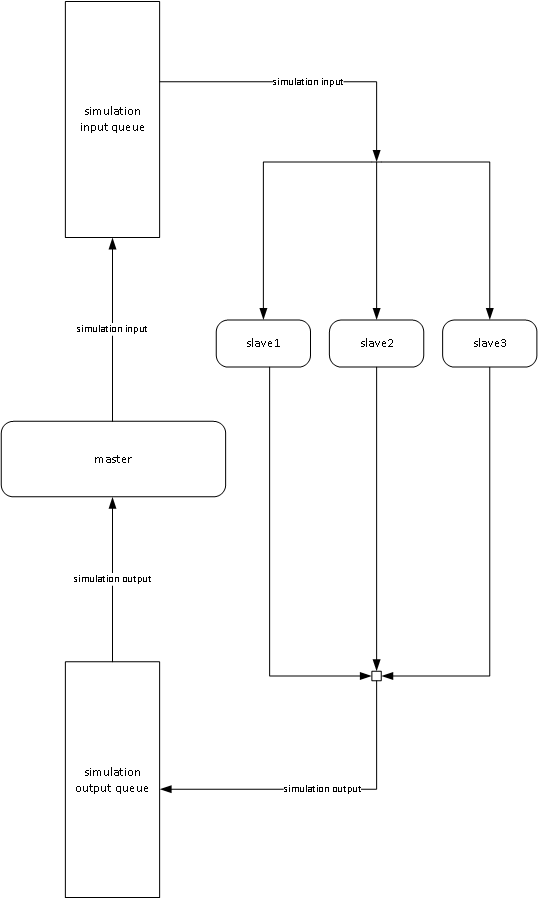
\includegraphics[width=60mm]{master-slave-queue.png}
\caption{Communication via FIFO Queue}
\end{figure}

In this way, communication cost inside single machine is dramatically reduced for both master and slaves.Except from the performance benefit it has brought in, adopting FIFO queues also helps to decouple the master and slaves, which makes the design more clear.

\subsubsection{Integrating R\&S Procedure}

As the simulation experiment is called through an abstract programming interface in slave, in master the R\&S procedure is also dealt in this way. The implementation of self-customized R\&S procedure should follow the specification, or function signature below:

\begin{lstlisting}[language=Java]
public int ras(double[][] alts,double[] args,SimHelper helper);
\end{lstlisting}

Here the first function argument $alts$ stands for all the alternatives. Noticed that it is an two-dimension array and each alternative is fully represented by an one-dimension array inside. For instance, in the (s, S) inventory problem, an alternative could be fully represented by two parameters $s$ and $S$ inside that one-dimension array. Usually a programmer would like to add an extra $id$ as the first parameter representing the alternative for convenience.

The second function argument $args$ stands for the parameters needed to carry out the R\&S procedure. For example, in the Rinott's procedure it will contain $\alpha$, $\delta$ and $n_0$. Programmer should arrange these parameters in this array.

The third function argument helper is a self-defined type, or class in Java, which contains all the needed callable programming interfaces, or pre-build-in functions for implementing a self-customized R\&S procedure.

The return value is the id of the selected alternative.

Now we introduce the programming interfaces provided for implementing R\&S procedures. Firstly let's look at two plain old Java objects, or POJOs for shout, which act like the struct in C-programming language. They are the wrappers for simulation input and output, so we name them as $SimInput$ and $SimOutput$, respectively. We only list the fields here, and will explain the meaning of each field later during the explanation of programming interfaces.

\begin{lstlisting}[language=Java]
public class SimInput {
	public int syncID;
	public int altID;
	public double[] args;
	public long[] seed;
}
\end{lstlisting}

\begin{lstlisting}[language=Java]
public class SimOutput {
	public int syncID;
	public int altID;
	public double[] result;
}
\end{lstlisting}

As for the programming interfaces for implementing R\&S procedures, they can be divided into two types, one is synchronized interfaces, the other is asynchronized ones.

Generally speaking, programming interfaces, or functions, which appear in pure serial program, are all synchronized. It means that once this function is called, the whole program will "stuck" there until the execution of that function is finished and the result get returned if there exits any.

On the contrary, interfaces appeared in parallel program may be synchronized or asynchronized. Asynchronized means that once the function is called, the function will return almost immediately, without the real execution. The real execution may be delayed to some point later, or may get started already but not yet finished. The caller of this asynchronized function may get informed of the execution result in the future, or may have to make polling request itself to get latest execution status.

The only synchronized interface is provided as:

\begin{lstlisting}[language=Java]
public SimOutput[] sim(int[] altIDs);
\end{lstlisting}

Here the only parameter $altIDs$ is the list of ids of alternatives need to be simulated against, each for once. Duplicated ids appeared in this array is allowed for replicated execution of simulation.

For example, during the implementation of the Rinott's procedure, this interface should be called twice, say, each in one stage. In the first stage the length of this array should be $kn_0$, standing for simulating against all the $k$ alternatives for $n_0$ times. As for in the second stage, the length of this array should be dependent on the result of first stage.

The return value here is an array of $SimOutput$ and each $SimOutput$ stands for the result of one simulation experiment. The order inside this array can be totally different from that in the input $altIDs$ array, which doesn't matter since the $altID$ field is exactly the one from the input $altIDs$ array. The result field will contain the simulation result, using an array to support multiple result values from simulation experiment.

Still in the example of the Rinott's procedure, since this interface is synchronized, it won't return until all the simulation results are ready, which archives an implicit barrier here. In this way, the classic two-staged Rinott's procedure can be fully implemented with this synchronized interface.

To support parallelism in fully sequential procedures, asynchronization is provided through at least two interfaces. One is for sending out simulation requests, the other is for collecting simulation results.

The asynchronized interface for sending out simulation request is provided as:

\begin{lstlisting}[language=Java]
public int asyncSim(int[] altIDs);
\end{lstlisting}

Here the only parameter $altIDs$ is the same meaning as that in the synchronized interface, while it will return immediately with an single int value representing an internal identification for synchronized simulation batch. This value will be used in implementing future procedure.

After calling this interface, the procedure can do what ever it needs to do, or call the asynchronized interface for collecting simulation result, which is provided as:

\begin{lstlisting}[language=Java]
public SimOutput[] takeSimOutputs(int n, boolean block);
\end{lstlisting}

Here the first parameter n is the number of simulation result demanded by caller, the second parameter block is a bool variable with following logic: If this variable is set to true, then this function will not return until n simulation result are ready for taken. Otherwise if this variable  is set to false, then this function will always return immediately no matter the n simulation result is ready. It is possible that only several simulation results are return with the number smaller than n, or no result get returned at all. Caller of this function can judge the situation from the return value.

A typical example of using these asynchronized interfaces is the implementation of the revised fully sequentially procedures. After sending out a certain number of simulation experiment requests, calling $takeSimOutputs$ with $n = 1$ and $block = true$ repeatedly, meaning that the fully sequential procedure could do something after each new sample value. The appending simulation requests are also sent out here, archiving customized sampling rule.

\subsection{Agent}

\subsubsection{Scale Out to Cluster}

With a limited number of slave threads inside a single machine, it is enough to have master and slave, but it's still very far way from reaching the bottle neck of the single master structure. In other words, we can get more speed up by simply adding slaves threads.

However, the maximum number of slave threads is empirically limited by the total number of hardware cores on that machine. We can definitely add more slave threads, but without enough hardware parallel executing units, namely cores, it is concurrency in fact, rather than real parallel. Adding more software threads than hardware executing units will hardly gain extra speed up, but will demand more scheduling effort from operating system.

Buying powerful machine with more hardware cores is an approach, which is named as scale up. However the price of the machine will grow much faster than linear against computing power, since the more the machine scales up, the higher technology it requires for manufacturing, which makes the cost increasing dramatically.

A common solution is to compose a cluster with several machines where each of them are not that powerful in single. This is called scale out. To make network communication efficiently, slaves communicate with the master via agent, except for those slaves running in the same machine as master. The agent will buffer the simulation input and output with FIFO queues, thus it is possible to make batched communication after scaling to a cluster, which is critical in network communication since with reliable connection-oriented protocol, establishing new connections frequently is much more costly than stable continues transportation.

\subsubsection{Buffering Policy}

In agent, we have two dedicated threads for managing buffered simulation input and output, respectively. The policy for input management is here:

\begin{algorithm}
\begin{algorithmic}[1]
\While{\text{true}}
  \If{$inputQueue.size() < s1$}
    \State{send one request for $(s2 - s1)$ simulation inputs via network}
    \ForAll{obtained simulation inputs}
      \State{inputQueue.put(input)}
    \EndFor
  \Else
    \State{sleep for 1 second}
  \EndIf
\EndWhile
\end{algorithmic}
\caption{Simulation Input Management in Agent}
\label{input_buf_alg}
\end{algorithm}

It is almost the $(s, S)$ inventory policy, and the two parameters can be specified manually. The $s$ should not be too small, otherwise some slaves may be idle due to lacking simulation input. We use the number of the slaves attached with this agent. Meanwhile, $S$ should not be too large, since it won't speed-up by pre-fetching too many simulation input, which only takes the risk fetching outdated input, which means that the corresponding alternative gets eliminated during the waiting in the buffer for so long.

The policy for output management is much more straightforward, just send out all the simulation output as soon as possible, because the earlier master can get these output, the more chance it gets to eliminate inferior alternatives. Currently this policy is perfectly okay since we don't use too many machines. If the number of agents or machines increases dramatically, we need to change this aggressive policy.

\subsection{User Interface}

In order to reduce the study cost of users who adopt our system, well designed user interface is necessary part in the whole system. In our system, the user interface can be divided into two kinds. One is for users using our system directly, the other is for users extending in ranking and selection procedure and simulation experiment.

For the first kind of user interface, we could simply leave a command line interface since it is only an academic purpose software tool. However, since at the end of day we would like it to become a computing service, or more precisely, cloud computing, which distributes computing service to end user via Internet, we developed a web interface for it, as a prototype for that stage. Here is a screenshot of that web page:

\begin{figure}[ht] \label{web-ui}
\centering
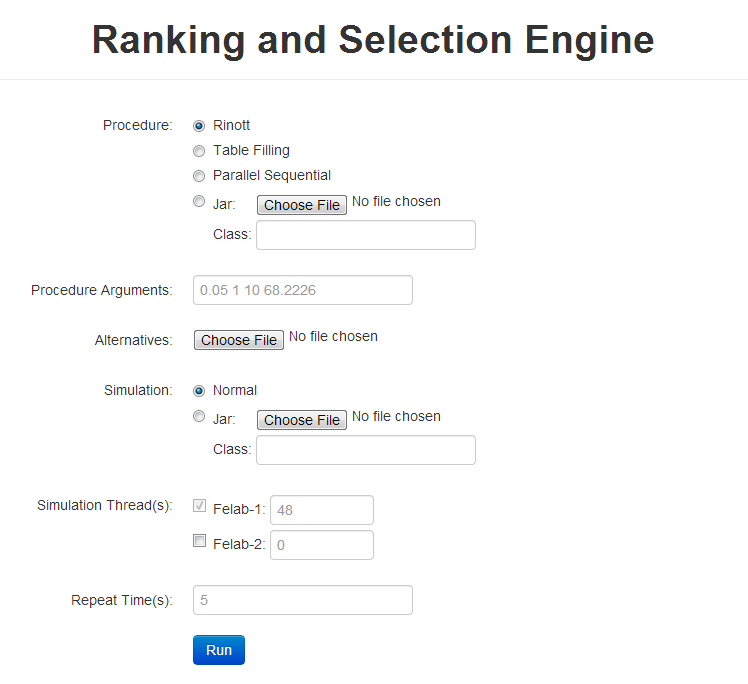
\includegraphics[width=120mm]{rase_web.png}
\caption{Web UI}
\end{figure}

In this way it is much more user friendly than command line. Beginning users could just choose corresponding R\&S procedure and simulation experiments and fill in the parameters intuitively, advanced users may develop his own simulation experiments, and professional users can develop his own procedure with fairly less effort than what he needs to spend without our work. Interested reader may refer to the appendix to get a detailed user guide of this web interface.

\section{System Evaluation}

In this section we will present the numerical results from the latest version of our system. We will start from listing the hardware and software environment of our experiment, then present the results when solving the three-stage buffer allocation problem, and finally give an analysis of the result.

\subsection{Hardware Environment}

Our experiment is done on a Dell PowerEdge R815 rack mount server, with four AMD Opteron 6176 CPUs equipped, namely a multi-processor machine. The total memory size is 64GB which is huge enough to support our experiment, and we will need to discuss the limitation from the number of hardware parallel execution units.

\subsubsection{Parallel Execution Units}

Each of the four AMD Opteron 6176 CPUs has 12 cores, thus 48 cores in total. Information from /proc/cpuinfo on operating system has also verified this hardware configuration.

Empirically it is possible to start more than 48 tasks at the same time. Besides, it is also quite proper since using up the computing ability of each machine is a way to reduce IT cost. Engineers in IT industry have even tried to study the most aggressive ratio of software parallel tasks over hardware parallel execution units, which highly depends on detailed scenario but is definitely no less than 1.

In our experiment, in order to guarantee an good parallel computing status among all slave threads, we set the number of slaves to 48 in maximum, which is quite conservative.

\subsection{Software Environment}

Commercial software components like the Windows from Microsoft or Matlab from Mathworks are not suitable for building systems which are going to scale out in the viewpoint of license cost, so we will build our implementation based on software that is free in charge.

\subsubsection{Operating System}

We have installed CentOS 6.2 as the operating system on our server, which is the most popular community supported and server oriented Linux distributions, and the name CentOS itself is short for "Community Enterprise Operating System".

CentOS is extremely stable since it has $100\%$ binary compatibility with its upstream source Red Hat Enterprise Linux, a ceremonially supported and enterprise server level Linux distribution from Red Hat, which is the leading Linux service provider in the world. 

\subsubsection{Run-time Environment}

We have installed Java Run-time Environment 1.6. We choose Java programming language since it is free compared to Matlab and powerful enough with abundant third-party libraries.

Extra benefit with Java includes but not limited to the natural ability of cross-platform, the robustness in the language itself, e.g..

\subsection{Numerical Result}

The numerical result is taken from solving a specific instance of the three-stage allocation problem with a fairly large scale. We have repeatedly run the experiments with different number of slave threads against this problem and finally have complete correctness and good parallelism archived.

\subsubsection{The Problem Scale}

The feasible region of this instance of three-stage allocation problem is defined as $x_1 + x_2 + x_3 \leqslant 20$, $x_4 + x_5 = 20$, $1 \leqslant x_i \leqslant 20$ and all the $x_i$ are natural number, so there are 21660 feasible solutions in total, in other words the $k = 21660$ here.

In previous time this scale size makes it thought as not suitable for solving by R\&S, and often dealt with through methods like OvS. In our experiment it is solved with an affordable time cost, which will be shown later.

\subsubsection{Correctness}

From the IZ viewpoint introduced before, both the best solutions and the ones which are within $\delta$ difference from the best solutions can be regarded as correct selection.

In this specific problem instance, all the correct selections can be obtained in advance through other methods, which let us to verify the correctness of results obtained from running our own R\&S implementation. The correct results are listed below:

\begin{table}[ht]
\begin{center}
\begin{tabular}{|c|c|}
\hline
Alternative & Comment \\
\hline
(6, 7, 7, 12, 8) & best \\
(7, 7, 6, 8, 12) & best \\
(6, 7, 7, 13, 7) & good \\
(7, 7, 6, 7, 13) & good \\
(6, 7, 7, 11, 9) & good \\
(7, 7, 6, 9, 11) & good \\
\hline
\end{tabular} \\
\caption{Results Obtained in Advance}
\end{center}
\end{table}

Again noticed that the best answers and the good enough answers are all considered as correct selection.

The corresponding log has shown that we archived correct selection every time running our implementation, regardless of different parallel configurations each time. This is also the basic requirement of our work. With the guaranteed correctness, we can focus on the performance data now.

\subsubsection{Performance}

Here we will report the total number of samples generated during R\&S and the total time spent during the whole program. The total number of samples can be regarded as total simulation workload approximately, which should be carried out by all the slaves in parallel. As for the total time cost, that is the most data we're interested in developing this implementation. Below is the detailed results:

\begin{table}[ht]
\begin{center}
\begin{tabular}{|c|c|c|c|c|c|c|}
\hline
Num. of Slaves(n): & 1 & 4 & 8 & 16 & 32 & 48 \\
\hline
Sample Size($\times 10^5$) & 2.426 & 2.434 & 2.442 & 2.442 & 2.433 & 2.436\\
\hline
Elapsed Minutes(t): & 370.5 & 129.4 & 94.4 & 68.3 & 41.7 & 34.2 \\
\hline
\end{tabular} \\
\caption{Performance Data}
\end{center}
\end{table}

The time cost reported in this time is at least affordable for research purpose now. By the way, we also monitored the program with a more professional tool named visualvm, interested reader may refer to the appendix.

\subsection{Performance Analysis}

We can see from the table above that the sample size varies very little from number of slaves, which implies that the simulation work load is almost fixed. According to Amdahl's law, the speed up ratio can be modeled as $\frac{1}{(1 - p) + \frac{p}{n}}$, where $p$ the parallel proportion of the program, $1 - p$ is the remaining serial proportion, and $n$ is the number of processors. Now we would like to estimate $p$ with model below:

$$ t = a \times (1 - p + \frac{p}{n}) + \epsilon $$

Here $a$ is the factor, $\epsilon$ is the noise, and we can get t and n from the result table above. The model can be turned into: 
$$ t = (a - ap) + ap \times \frac{1}{n} + \epsilon $$

With linear regression, we can get $a - ap = 40.4$ and $ap = 332.9$ with $R^2 \geqslant 0.994$, so $p$ is 0.892, which means 89.2\% of simulation work is paralleled.

This parallel ratio fits the R\&S feature that intuitively most workload can get executed in parallel, and also get benefited from all the design decisions and programming techniques with the purpose of reducing the serial workload. It can be considered as a good starting point of scaling out to more execution units, where a cluster rather a single machine will be involved.
